\documentclass{uva_bachelor_thesis}
\usepackage{hyperref} % for bibtex urls
\usepackage{csquotes} % for quotes
\usepackage[acronym, nonumberlist]{glossaries}
\usepackage{tikz}
\usepackage{newclude} % include without page break
\usetikzlibrary{positioning,%
  shapes.geometric,%
  shapes.misc,%
  calc,%
  fit,%
  decorations,%
  decorations.pathreplacing,%
  backgrounds,%
  arrows,%
  automata,%
  trees%
}

\xdefinecolor{bordeaux}{RGB}{128,0,50}
\xdefinecolor{niceblue}{RGB}{13,41,79}
\xdefinecolor{nicegreen}{RGB}{13,79,18}
\xdefinecolor{niceviolet}{RGB}{79,13,74}
\colorlet{maincolor}{niceviolet}
\colorlet{alertedcolor}{red}
\colorlet{examplecolor}{green!50!black}

% Glossary items
\makeglossaries
\newacronym{gui}{GUI}{graphical user interface}
\newacronym{mvc}{MVC}{model-view-controller}

% Title Page
\title{CLIsis: An Interface for Visually Impaired Users of Apache Isis Applications}
\author{Sander Ginn}
\supervisors{Maarten Marx (UvA), Dan Haywood (Apache)}
\signedby{Maarten Marx (UvA)}


\begin{document}
\maketitle

\begin{abstract}
This will be the abstract.
\end{abstract}

\tableofcontents

\chapter{Introduction}
\label{chapter:introduction}
Every application that offers a method of interaction with a human being requires some form of user interface to enable this interaction. But what exactly characterises a user interface? Galitz\cite{galitz2007essential} provides the following definition for 'user interface':
\begin{displayquote}
\textit{The user interface is the part of a computer and its software that people can see, hear, touch, talk to, or otherwise understand or direct.}
\end{displayquote}

Thus, in the context of an application, a user interface is a means of interaction between the user and system based on mutually understood communication methods. These communication methods can range from visual methods such as computer displays to audible methods like speakers. 

This is still a very abstract definition of what a user interface does. It does not specify how system information is presented, how the user provides input, what permissions and restrictions the interface must adhere to, et cetera. Nielsen\cite{nielsen1994usability} describes an overview of user interfaces throughout history which will provide some practical examples.

When the computer was in its infancy, several primitive user interfaces were developed. As the use of computers became more widespread, however, the \textit{line-oriented interface} was adopted as a method of interaction. The name is derived from the characteristic that the user interacted with a system on a single line; once submitted, the command could not be modified anymore. As long as the presented information is well structured this method of interaction still has valid use cases in present times, as it effectively delimits functionality and thus prevents novice users from running into issues. Assistive technology for visually impaired users excelled with line-oriented interfaces: as all content was character based, it could easily be made interpretable for someone who lacks (good) vision, for example through audio\cite{poll1996visualising}.

The successor of line-oriented interfaces is the \textit{full-screen interface}. This interface aims to exploit a greater deal of the screen real estate by enabling the user to interact with more elements than just one input line. The full-screen interface also introduced the concept of menus, where functionality available to the user is listed in a hierarchical structure. Menu design has been researched extensively to determine the optimal balance of depth and breadth\cite{paap1986optimal, landauer1985selection, fisher1990optimal}. Depth decreases complexity of menus while increasing ease of navigation; the contrary applies to breadth. However, menu-based interfaces also marked the beginning of a decrease in accessibility for visually impaired users, as the information displayed gradually became more catered towards a visual mental model. Visually impaired users tend to mentally model information differently, and thus directly translating a visual interface to a non-visual representation can be extremely difficult to comprehend for the target audience\cite{edwards1994providing}.

Finally, the user interface type which is currently the most widespread, is the \textit{\acrlong{gui}} (\acrshort{gui}). The vast majority of modern applications offer a graphical user interface as their primary method of interaction. A key characteristic of \acrshortpl{gui} is that interaction is offered through direct manipulation. Rather than issuing a command which exactly specifies those parameters of what has to happen, the user gets continuous feedback of their input commands. The obvious advantage of a \acrshort{gui} is that it can take advantage of the human sight to represent data in a more intuitive way. Research has shown that when the interface adheres to some fundamental principles, a user's cognitive performance increases with a \acrshort{gui}. An example of one of these principles is Miller's Law, proposed in his seminal research on information processing\cite{miller1956magical}. However, Nielsen also addresses the issue that motivates this research: a \acrshort{gui} sidelines the visually impaired from using an application.

Enabling the visually impaired to use applications despite a lack of or very bad vision has been an ongoing effort since \acrshortpl{gui} were widely accepted as the de facto standard\cite{boyd1990graphical}. However, it has proven to be difficult to design a \acrshort{gui} that is also accessible without visual cues. A big issue is that standardisation has proven ineffective: even though the United States has passed laws that enforce accessibility of websites\cite{Secti81:online} and the World Wide Web Consortium has developed the Web Content Accessibility Guidelines\cite{WebCo83:online}, research has shown that these guidelines are very often ignored and thus websites are rendered inaccessible for accessibility tools such as screen readers\cite{leuthold2008beyond}.

Visually impaired computer users often make use of a \textit{screen reader} to translate visual objects into a representation that can be interpreted by assistive technology, such as braille terminals or text-to-speech. However, Lazar et al. found that 4 out of 5 top causes of frustration for blind users of screen readers were related to poor design choices of the software or website developer\cite{lazar2007frustrates}. As a solution to these problems, we will implement a bespoke interface that does not require the use of a third party screen reader.

This research aims to provide an alternative interface for visually impaired users for applications developed with the Apache Isis\cite{Apach60:online} framework. This interface will not serve as a replacement for the existing interface nor blend in with it. The interface is derived from the metamodel of the framework and thus content unaware. This means that the interface is readily available for any Isis application and no alterations are necessary to add it to an existing application.

\section{Research questions}
\label{section:researchquestions}
The central research question in this thesis is:

\MyQuote{Can a content unaware graphical user interface be adapted to a non-visual interface so that visually impaired users are able to interact with the application?} \label{RQ1}

\noindent For the non-visual interface to be useful it is imperative that it offers the same functionality as the graphical user interface. Therefore, we will also answer the following subquestion:

\MyQuote{When implementing a non-visual interface, can the integrity of the domain model be maintained while providing an effective and simple method of interaction?} \label{RQ2}

\noindent Finally, it is desired that the non-visual interface does not severely impact user performance, as this would imply that it is not a legitimate alternative to the existing interface. Thus, a second subquestion will be answered:

\MyQuote{Compared to the standard interface, how is performance affected when the user employs the new interface?} \label{RQ3}

\section{Overview of thesis}
\label{section:overviewofthesis}
First, chapter~\ref{chapter:theoreticalbackground} will describe the philosophy of Apache Isis, other efforts in improving accessiblity for visually impaired users, and issues that arise when a user interface is adapted. Chapter~\ref{chapter:methods} then outlines what methods are used to perform the adaptation and evaluation of the new user interface. The implementation is explained in chapter~\ref{chapter:implementation}. Chapter~\ref{chapter:evaluation} assesses the final product and presents the results of the experiments. Finally, chapter~\ref{chapter:conclusion} answers the research questions based on the findings in chapter~\ref{chapter:evaluation}.
\chapter{Theoretical background}
\label{chapter:theoreticalbackground}
User interface design is a thoroughly studied discipline with strong roots in psychology. In the 1980s \acrshort{gui} development exploded due to better hardware\cite{myers1998brief}. This meant that traditional user interfaces had to be redesigned to accommodate to the graphical features of the modern computer. In section~\ref{section:userinterfacemigrationinhistory} we will provide a brief history on how this was achieved and what sort of issues arose when migrating a user interface. Furthermore, section~\ref{section:apacheisis} will describe what Apache Isis entails.

\section{Apache Isis}
\label{section:apacheisis}
As a software engineer, picking a framework for developing web applications can be a tedious process. There are dozens of frameworks for Java alone, with the oldest and most adopted one being Spring\cite{Sprin96:online}. The vast majority of these frameworks are based on the \textit{\acrlong{mvc}} (\acrshort{mvc}) pattern, where the view displays information to the user, the controller processes interaction between the user and the view, and the model contains the information and logic that manipulates this information\cite{leff2001web}. The relations between the components are depicted in figure~\ref{figure:mvc}.

While the \acrshort{mvc} pattern itself has a lot of advantages, it has received criticism in the context of web development. The concept of separating business logic from presentation logic is often not adhered to in web applications, resulting in controllers that are contaminated with logic that should live in the model\cite{Fulfi2:online}.

\begin{figure}[h]
	\center
	\include*{figures/mvc}
	\caption{Interaction between the components of an MVC application}
	\label{figure:mvc}
\end{figure}

This is where Apache Isis differs from more classic \acrshort{mvc}-based frameworks. There is no need for an explicit controller layer, as the core strength of the framework is that behaviour which would normally be defined in controllers is automatically generated by reflection\footnote{Reflection is a language's ability to inspect and dynamically call classes, methods, attributes, etc. at runtime.}. A major benefit of this feature is that prototyping is greatly simplified; the business logic is virtually all that needs to be programmed, and the framework does the rest. This means that project managers, product owners and other parties involved can be presented with working prototypes rather than charts and specifications, and it relieves developers from wasting precious time on coding the visible part of an application - code which often has limited reusability in a later stage of development.

This does not, however, imply that Apache Isis is merely useful for prototyping. The automatically generated interface is perfectly suitable for a lot of business oriented applications. Estatio\cite{Estat40:online}, an estate management application built on Apache Isis commissioned by a listed real estate investment firm, makes use of the standard wicket viewer. In case a given application demands a bespoke user interface, it can be designed to use the \acrshort{rest} API which ships with Apache Isis, which we will use to implement our interface. Furthermore, there are nearly thirty add-ons available which can be plugged into any Apache Isis application\cite{Apach4:online}, which offer various features such as Excel spreadsheet importing. Finally, the framework takes testing support very seriously, offering unit and integration testing functionality to ensure the business logic behaves as expected.

Apache Isis is developed on two fundamental philosophies: domain-driven design and the Naked Objects pattern.

\noindent
\begin{figure}
\begin{minipage}{.5\textwidth}
\begin{javacode}
@DomainObject
public class SimpleObject implements Comparable<SimpleObject> {
    public TranslatableString title() {
        return TranslatableString.tr("Object: {name}", "name", getName());
    }

    @javax.jdo.annotations.Column(
            allowsNull="false"
    )
    
    @Property
    @Getter @Setter
    private String name;

    public TranslatableString validateName(final String name) {
        return name != null && name.contains("!") ?
            TranslatableString.tr("Exclamation mark is not allowed"): null;
    }
}
\end{javacode}
\end{minipage}
\begin{minipage}{.5\textwidth}
	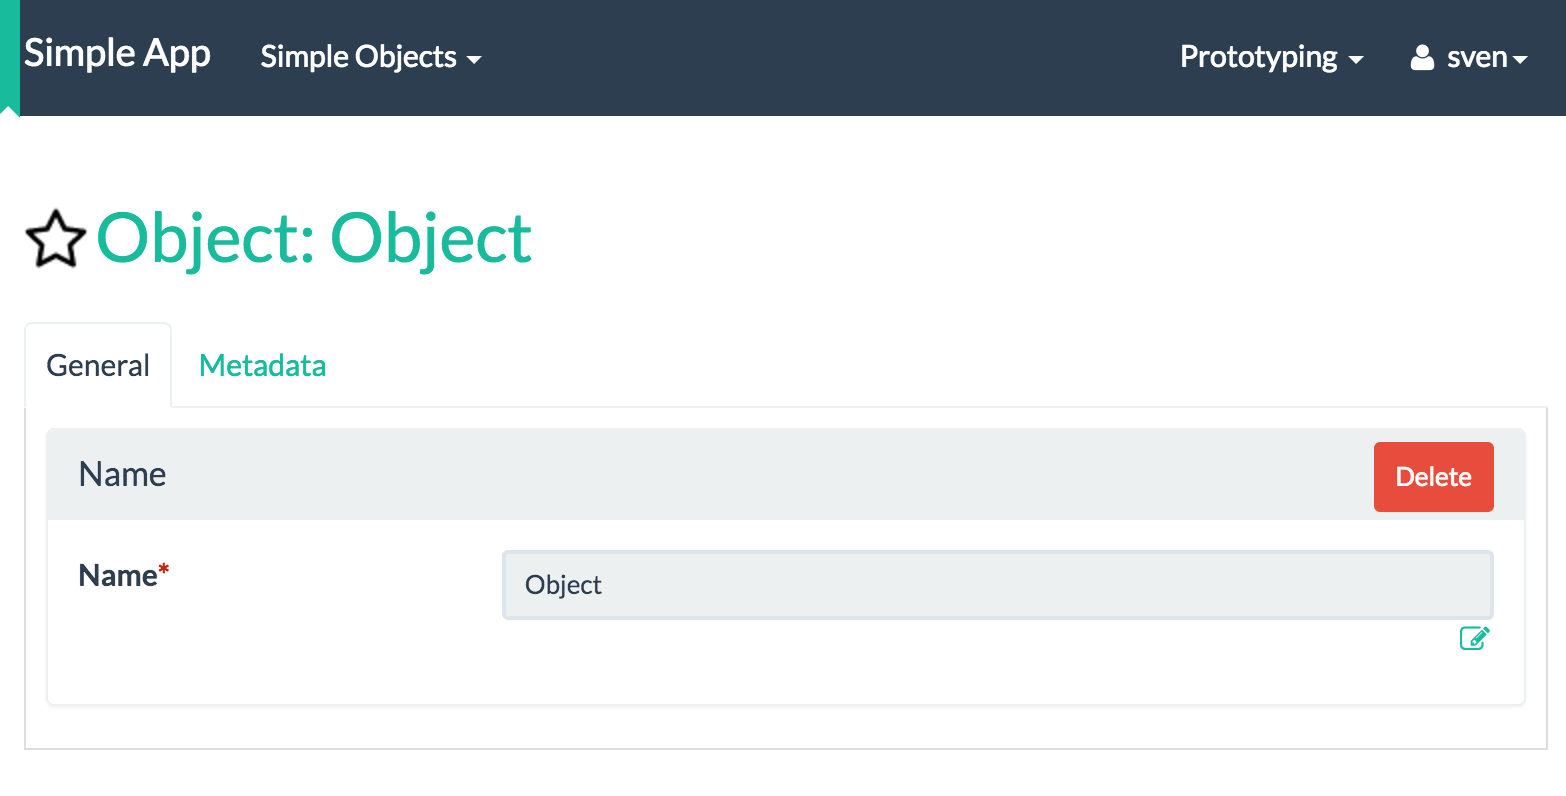
\includegraphics[width=\textwidth]{figures/simpleobjectui}
\end{minipage}
\caption{A very simple example of how the user interface is derived from code}
\end{figure}

\subsection{Domain-Driven Design}
\label{subsection:domaindrivendesign}
Software projects have been riddled by failure for as long as they have been around. A 1999 survey by Linberg found that 20\% of software projects failed and another 46\% suffered from severe delays, exceeding budgets or missing functionality or a combination of the three\cite{linberg1999software}. In 2007, the Standish Group concluded that 35\% of software projects could be classified as successful, with 46\% suffering from the aforementioned problems and 19\% completely failing\cite{rubinstein2007standish}. Keil et al. concluded that a key factors in the failure of software projects are information asymmetry and goal incongruence\cite{keil2000software}.

Those exact issues are at the core of what \textit{\acrlong{ddd}} (\acrshort{ddd}), conceived by Eric Evans in 2004, encapsulates. In a business software project, there are two main parties involved: the domain experts (the business experts) and the technical experts (the developers). These parties will have to work together in order to specify the functionality of the software. Business language, however, is very different from technical language, and thus some method of translation is needed. A business analyst could provide this translation, but this only adds another layer of potential misunderstanding, ultimately culminating in faulty behaviour being implemented.

\subsubsection{Ubiquitous language}
\label{subsubsection:ubiquitouslanguage}
The first central concept in \acrshort{ddd} is to create an \textit{ubiquitous language} between the domain experts and technical experts. By clearly defining what terms to use for what concepts and ensuring that both parties understand what they mean, information asymmetry can be avoided\cite{evans2004domain}. These defined terms together form the domain model which is used to describe and specify the software. Undoubtedly, at some stage in the process the ubiquitous language will prove itself insufficient to accurately describe new functionality, which implies that the model should be expanded. This creates an iterative development process where both parties have to put in effort to be as concise as possible. It also prevents the domain model from growing too complex: if the parties fail to define a certain aspect of the model, it is highly unlikely that it will be successfully implemented in the software and it is better to leave it out.

\subsubsection{Model-driven design}
\label{subsubsection:modeldrivendesign}
Once the domain model has been specified to a sufficient extent to initiate the development process, the second central concept in \acrshort{ddd} comes to light: \textit{model-driven design}. As the name suggests, this means writing your software driven by the domain model. The domain model will function as the translation layer between the domain experts and the technical experts, as the software becomes more comprehensible for the domain experts if the software uses the same ubiquitous language. The code and domain model share a bidirectional relationship: if the domain model is extended, the code must be changed, and if the code is changed, the domain model must be adapted\cite{evans2004domain}. This prevents the issue of goal incongruence, as the domain experts and technical experts are aligned in terms of what has to be implemented. After all, the domain model is binding and defined in a collaborative effort.

\subsection{Naked Objects pattern}
\label{subsection:nakedobjectspattern}
One of the frustrations often expressed regarding \acrshort{ddd} is that while the ubiquitous language combined with the derived domain model may very well tackle the problem of goal diversion, it also increases overhead greatly. Consider figure~\ref{figure:applicationlayers}: the domain model is represented in the business logic layer. Recall that we've stated that the domain model will be refined over the course of time, and that any changes to the domain model must be reflected in the code. This means that any modifications to the domain model will have to be applied to the other layers, too.

\begin{figure}[h]
	\center
	\include*{figures/applicationlayers}
	\caption{The main application layers in \acrshort{ddd}}
	\label{figure:applicationlayers}
\end{figure}

To address this issue, Richard Pawson designed the Naked Objects pattern, based on three core concepts\cite{pawson2002naked}:
\begin{enumerate}
	\item Business logic should only reside in domain objects\footnote{A domain object is an entity that holds relevant data, in order to transfer the data between the application layers.}
	
	\item The user interface is an exact representation of the domain objects, and thus is an object-oriented user interface
	
	\item The user interface is derived completely and fully automatically from the domain objects through reflection
\end{enumerate}

These three concepts combined provide a means of developing software that robustly follows the philosophy of \acrshort{ddd}. The first two concepts ensure that the software implements the domain model and prevents the use of technical language. The application, whether prototypal or deployed, will feel familiar to the stakeholders and developers alike. The third concept is not necessarily related to \acrshort{ddd}, but does take away the burden of developing the presentation layer and thus places the focus on the business logic: i.e., the domain model.

\section{User interface migration in history}
\label{section:userinterfacemigrationinhistory}
In the history of user interfaces, two events stand out: the migration from character-based interfaces to graphical interfaces, and implementing a web-based interface for a native application.

As the use of \acrshortpl{gui} became widespread, a lot of older software still made use of legacy user interfaces. These interfaces were usually character-based interfaces, developed for hardware that did not offer the capabilities to use a \acrshort{gui}\cite{merlo1995reengineering}. Developers quickly came to notice that the migration of one user interface to the other was not easily accomplished, as end users wanted novel user interfaces to have identical functionality as the legacy counterpart, and a lack of homogenisation in hardware support resulted in a vast amount of code refactoring to achieve the desired result\cite{moore1994knowledge}. On top of that, simply redesigning the software from scratch would be an effort too costly in terms of resources and investments. As a result, the developers often reverse engineered the system, creating an object-oriented model and then wrapping the legacy objects so that the new system could use these entities\cite{de1997migrating}. This method allowed developers to incrementally phase out parts of the software until all legacy objects were removed.

Another major shift in user interface design came to the forefront when the internet was adopted in offices and homes alike and applications started to become available in the web browser rather than a native application for independent operating systems. This migration is still taking place to this day; an example is Skype, of which Microsoft introduced a preview version of its web based version as late 2013\cite{TypeL20:online}. Developers now had to deal with writing the presentation layer in all-new web technologies which run client side, while respecting the many constraints dictated by the software. When the underlying logic is not too complex, developers usually opted for "grafting" the web interface on top of the application, designing most of the mutually indepent functionalities from scratch and applying reverse engineering where necessary. For more complex applications, however, a comparable wrapping method as mentioned before could also be employed\cite{aversano2001migrating}.

Developers often also face the common issue of "dead" or "glue" code when migrating legacy systems to a web version, requiring the developers to thoroughly analyse code to prevent obsolete functionality from being implemented in the new user interface. Moreover, partially reusing code modules may also violate application logic\cite{stroulia2003user}. Finally, the great advantage of web availability of software is that it becomes accessible to a vast group of users: e.g. a bank offering web-based banking to its customers, removing the need of trained bank clerks. This does, however, introduce another layer of complexity, as the various groups of users should interact with the user interfaces designed for them - corporate clients require more functionality than a personal customer, but they both speak to the same back end\cite{aversano2001migrating}.
\chapter{Methods}
\label{chapter:methods}
We have selected several methods for implementing the new interface. First, section~\ref{section:userinterfaceadaptation} will describe the method applied to the existing interface in order to form a theoretical basis for the implementation. Section~\ref{section:experiments_methods} then outlines what experiment methods are used to evaluate the interface.

\section{User interface adaptation}
\label{section:userinterfaceadaptation}
Adapting an existing user interface to a new version has been described extensively\cite{classen1997cui, csaba1997experience, kong2000legacy}, but virtually all research that concretely describes the legacy and novel user interface aims at implementing a 'next generation' user interface, whereas our goal could be interpreted as moving back one generation, as we will remove any visual aspects from the existing interface. Therefore, we have opted to apply a more abstract method of adapting a user interface.

In \textit{Issues in User Interface Migration}, Moore describes migration as \textit{"the activity of moving software away from its original environment, including hardware platform, operating environment or implementation language to a new environment"}\cite{moore1993issues}. Although not all of these characteristics apply to our situation, the article proposes a method for systematic user interface migration that fits our purpose. The migration process is partitioned in three stages which are each described in subsections~\ref{subsection:detection},~\ref{subsection:representation} and~\ref{subsection:transformation}.

\subsection{Detection}
\label{subsection:detection}
The first stage of the migration process is the detection stage. The goal of this stage is to identify user interface functionality in the existing code through analysis. Moore lists several techniques that can be applied to perform the analysis:

\begin{enumerate}
	\item \label{item:patternmatching} Pattern matching of an abstract syntax tree that is created by parsing source code
	\item \label{item:syntacticanalysis} Syntactic/semantic analysis of the source code against predefined keywords that identify user interaction 
	\item \label{item:manualdetection} Manual detection of the source code 
\end{enumerate}

The article rightfully stresses issues that might arise when utilising technique~\ref{item:manualdetection}, such as the likelihood of introducing errors and an insurmountable amount of time necessary to perform the detection. This certainly holds true in situations where a content specific user interface is going to be migrated, and (partially) automated techniques such as~\ref{item:patternmatching} and~\ref{item:syntacticanalysis} will prevent these issues to a great extent. Our research question, however, is focused on adapting a content unaware user interface and thus analysing the user interface of a specific application developed with Apache Isis is pointless, as there is no reassurance that any functionality found in this application is relevant to other applications. This invalidates techniques~\ref{item:patternmatching} and~\ref{item:syntacticanalysis} in our research scope.

Fortunately, due to the property of Apache Isis that the user interface is automatically generated through reflection, functionality in the user interface can be described in a more abstract form. This reduces the size of the user interface ontology to such an extent that manual detection can be deemed a feasible technique for the detection stage. Furthermore, all relevant features are well-documented\cite{Docum42:online} and thus it can be verified that the detection results are complete and correct.

We performed manual detection on the framework which resulted in the following functionality to be exposed:

\begin{itemize}
	\item 
	\textbf{Menus} \\
	A user can access menus in the interface. Menus are available at any point in the interface.
	
	\item
	\textbf{Actions} \\
	A user can invoke menu and object actions.
	
	\item
	\textbf{Action prompts} \\
	If an action requires parameters, a user can enter the parameters in an action prompt.
	
	\item
	\textbf{Objects} \\
	A user can access objects and their properties.
	
	\item
	\textbf{Parented collections} \\
	A user can access collections that display objects related to a single object.
	
	\item
	\textbf{Standalone collections} \\
	A user can access collections that display objects, e.g. when an invoked action returns multiple objects.
\end{itemize}

These six elements together comprise the entire abstract user interface ontology. Figure~\ref{figure:uml} illustrates the relationships between the individual elements.

\begin{figure}
	\center
	\includegraphics[width=\textwidth]{figures/uml}
	\caption{UML representation of the abstract user interface ontology}
	\label{figure:uml}
\end{figure}

With the detection stage complete, we move on to the second stage.

\subsection{Representation}
\label{subsection:representation}
The second stage of the migration process is the representation stage. The objective of this stage is to describe and document the functionality that we uncovered in the detection stage. It must be described in such a way that it is not dependent on the target platform or technology while still adequately representing all requirements of the user interface.

We have drafted a set of specifications which represent the functionality which our new interface must implement. This stage is particularly relevant to answering research question~\ref{RQ2}, as it allows us to judge whether or not the domain model is still intact; successfully implementing all specifications implies that the integrity of the domain model is maintained.

\newpage
\noindent
\small

\begin{tabularx}{0.49\textwidth}[t]{lX}
	\toprule
	\multicolumn{2}{c}{\textbf{Specification S1}} \\
	\midrule
	\textbf{Description} & Menus can be accessed at all times \\
	\addlinespace[0.5em]
	\textbf{Rationale}	 & Classes annotated with \texttt{@DomainService} are menus in the \acrshort{gui}. In the new interface menu selection will be the first user interaction and menus are available at any point in the interface. \\
	\bottomrule
\end{tabularx}\hspace{0.02\textwidth}
\begin{tabularx}{0.49\textwidth}[t]{lX}
	\toprule
	\multicolumn{2}{c}{\textbf{Specification S2}} \\
	\midrule
	\textbf{Description} & Objects can be accessed \newline \\
	\addlinespace[0.5em]
	\textbf{Rationale}	 & Classes annotated with \texttt{@DomainObject} are objects in the \acrshort{gui}. Any object that is available in the \acrshort{gui} must be accessible in the new interface. \newline \newline \\
	\bottomrule
\end{tabularx}
\\[1em]

\begin{tabularx}{0.49\textwidth}[t]{lX}
	\toprule
	\multicolumn{2}{c}{\textbf{Specification S2-A}} \\
	\midrule
	\textbf{Description} & Object properties can be accessed \\
	\addlinespace[0.5em]
	\textbf{Rationale}	 & Object variables annotated with \texttt{@Property} are properties of this object, such as names or dates. In the new interface, primitive properties must be visible and object properties must be accessible.\\
	\bottomrule
\end{tabularx}\hspace{0.02\textwidth}
\begin{tabularx}{0.49\textwidth}[t]{lX}
	\toprule
	\multicolumn{2}{c}{\textbf{Specification S3}} \\
	\midrule
	\textbf{Description} & Collections can be accessed \newline \\
	\addlinespace[0.5em]
	\textbf{Rationale}	 & Variables annotated with \texttt{@Collection} are collections in the \acrshort{gui}. Collections should be displayed correctly depending on if they are parented or standalone (see figure~\ref{figure:uml}) and all objects must be accessible. \\
	\bottomrule
\end{tabularx}
\\[1em]

\begin{tabularx}{0.49\textwidth}[t]{lX}
	\toprule
	\multicolumn{2}{c}{\textbf{Specification S4}} \\
	\midrule
	\textbf{Description} & Actions can be executed \newline \\
	\addlinespace[0.5em]
	\textbf{Rationale}	 & Functions annotated with \texttt{@Action} are operations on a certain entity in the application, such as executing a search query. Any action that is available in the \acrshort{gui} must be available in the new interface. \\
	\bottomrule
\end{tabularx}\hspace{0.02\textwidth}
\begin{tabularx}{0.49\textwidth}[t]{lX}
	\toprule
	\multicolumn{2}{c}{\textbf{Specification S4-A}} \\
	\midrule
	\textbf{Description} & Action parameters can be accessed \\
	\addlinespace[0.5em]
	\textbf{Rationale}	 & Actions may have parameters necessary to execute them. These parameters must be accessible. \newline \newline \newline \\
	\bottomrule
\end{tabularx}
\\[1em]

\begin{tabularx}{0.49\textwidth}[t]{lX}
	\toprule
	\multicolumn{2}{c}{\textbf{Specification S5}} \\
	\midrule
	\textbf{Description} & A help menu can be accessed at all times\\
	\addlinespace[0.5em]
	\textbf{Rationale}	 & Users must be able to get context-specific help at any point in the interface. \\
	\bottomrule
\end{tabularx}\hspace{0.02\textwidth}
\begin{tabularx}{0.49\textwidth}[t]{lX}
	\toprule
	\multicolumn{2}{c}{\textbf{Specification S6}} \\
	\midrule
	\textbf{Description} & The application can be terminated \\
	\addlinespace[0.5em]
	\textbf{Rationale}	 & The user must be able to log out and exit the application. \newline \\
	\bottomrule
\end{tabularx}
\\[2em]

\begin{tabularx}{0.49\textwidth}{lX}
	\toprule
	\multicolumn{2}{c}{\textbf{Specification S7}} \\
	\midrule
	\textbf{Description} & The application provides error handling \\
	\addlinespace[0.5em]
	\textbf{Rationale}	 & The framework offers a lot of error feedback, such as invalidation messages after incorrect parameters. The new interface must provide a method of handling errors. \\
	\bottomrule
\end{tabularx}

\normalsize

\subsection{Transformation}
\label{subsection:transformation}
The third and final step in the migration process is the transformation step. We found ourselves in a similar situation as in the representation step; Moore describes a number of (partially) automated techniques to perform the transformation, often relying on generating code based on mappings between a specific type of representation such as XML and the detection stage results. Again, this is tailored towards content-aware user interfaces, and thus we will simply use a manual transformation as our user ontology is concise enough to do so.

The actual transformation stage is described in detail in chapter~\ref{chapter:implementation}.

\section{Experiments}
\label{section:experiments_methods}
To answer research question~\ref{RQ3} and subsequently research question~\ref{RQ1}, we will conduct a series of experiments to evaluate how user performance differs from the standard user interface when the new user interface is used. First, a theoretical approach is taken by applying the GOMS method, which we will describe in section~\ref{subsection:goms_methods}. Some limitations apply to this method, however. To compensate for these limitations we will run time trials with a set of test subjects to obtain empirical results, as explained in section~\ref{subsection:timetrial_methods}. The results of these experiments are covered in chapter~\ref{chapter:evaluation}.

\subsection{GOMS}
\label{subsection:goms_methods}
The \textit{\acrlong{goms}} (\acrshort{goms}) method is a well-established method to model efficiency-related design issues and is often applied in early stages of user interface design evaluation\cite{schrepp1990goms, john1996goms, kieras1994goms}. It is a qualitative method that aims to predict user execution time of a goal-oriented task. There are four individual components:

\begin{itemize}
	\item The \textbf{goal} is what is expected of the user to accomplish in the task
	\item The \textbf{operators} are physical and cognitive processes that are required to complete the task
	\item The \textbf{methods} are series of operators that the user can execute to reach the goal
	\item When there are multiple methods to achieve the same goal, the \textbf{selection rules} will decide which method is picked
\end{itemize}

Physical operators are processes such as moving the mouse to a target destination or pressing a key, whereas processes like deciding between two options and remembering previous information are examples of cognitive operators. For more accurate results, it is recommended to determine the operator time coefficients empirically in a controlled environment which resembles the context of the \acrshort{goms} analysis\cite{gong1994validation}. We are unable to do so within the timeframe of this research and thus will apply the coefficients posed by the inventors of the method, which have been adopted more universally\cite{kieras2001using}:

\begin{itemize}
	\item \textbf{K - keystroke}: .28 seconds for an average nonsecretarial typists
	\item \textbf{T$_n$ - sequence of \textit{n} characters}: n $\times$ K seconds
	\item \textbf{P - point with mouse to target}: 1.1 seconds
	\item \textbf{B - press mouse button}: .1 seconds
	\item \textbf{H - home hands to keyboard or mouse}: .4 seconds
	\item \textbf{M - mental act of routine thinking or perception}: 1.2 seconds
\end{itemize}

Research has shown that typing accuracy of visually impaired users is not significantly different from sighted users\cite{ishida1993accuracy}, and thus we will use the average speed for keystrokes.

The advantages of \acrshort{goms} analysis are that it is a fast and cheap way of obtaining results. It does, however, have several limitations that must be kept in mind\cite{schrepp1990goms}. First, the model applies to expert users and execution times are thus based on users who are familiar with the system; novice users will usually perform worse than the projected time. Second, it does not account for errors which in reality will occur. Third, it can only apply to serial execution of tasks, excluding parallel tasks from the analysis. Finally, it does not take user fatigue in account which will increase during extended usage.

\subsection{Time trial}
\label{subsection:timetrial_methods}
To attain empirical results regarding user performance in the new interface, we will compose 5 test scenarios that will be executed by a small number of test subjects. All scenarios will be executed in both user interfaces, where we will avoid bias by providing them out of order and alternating between the user interfaces\cite{chen2007comparing}. All user interaction will be captured to enable analysation of every step that is required to fulfill the tasks.

To log the user interaction in the standard interface, we will use an adapted form of Apache Isis' \texttt{PublisherServiceLogging} class. This is a built-in module to publish events such as action invocations or property changes to a logfile. A small adaptation was made to include logging of events such as the loading of objects or typing in a parameter field.

Since the new user interface will only have one input field that is permanently in focus, all user interaction will be confirmed with pressing the enter key. This allows us to print the input text with a timestamp, logging all user interaction.

For each step, we can then take the mean of time it took for each participant to get to the next step, up until completion of the task. By plotting a timeline for both user interfaces and their respective means, we will be able to visualise the performance difference between the user interfaces in a clear manner.
\chapter{Implementation}
\label{chapter:implementation}
This chapter describes the practical side of the project. 

\section{Frameworks and tools}
\label{section:frameworkandtools}
This section expands on what available software tools I have used to implement the new interface.

\subsection{REST API}
\label{subsection:restapi}
This subsection will describe how Apache Isis' REST API works and how it is incorporated in the new interface.

\subsection{AngularJS}
\label{subsection:angularjs}
Here I will explain the choice for AngularJS.

\subsection{Web Speech API}
\label{subsection:webspeechapi}
This subsection will describe how the Web Speech API is used.

\section{Functionality}
\label{section:functionality}
This section will expand on the individual components that process the information from the REST API.

\subsection{Main module}
\label{subsection:mainmodule}
This subsection describes the main app module.

\subsection{Controllers}
\label{subsection:controllers}
This subsection describes each controller's functionality.

\subsection{Views}
\label{subsection:views}
This subsection describes the purpose of each view.
\chapter{Evaluation}
\label{chapter:evaluation}
This chapter describes the experiment results and answers the research questions.

\section{Specification requirements}
\label{section:specificationrequirements}
In this section, I will motivate which specifications have been met in the implementation. With this information I will be able to answer the first subquestion.

\section{Experiments}
\label{section:experiments_evaluation}

\subsection{GOMS}
\label{subsection:goms_evaluation}
Here, the results from applying GOMS will be evaluated.

\subsection{Time trial}
\label{subsection:timetrial_evaluation}
Here, the results from the time trial experiment will be evaluated.

\subsection{Performance difference}
\label{subsection:performancedifference}
This subsection will evaluate the experiment results and answer the second subquestion.

\chapter{Conclusion}
\label{chapter:conclusion}
To conclude this research, we will assess the achieved results in relation to each research question. Research question~\ref{RQ3} can be answered first:

\begin{displayquote}
	\textit{Compared to the standard interface, how is performance affected when the user employs the new interface?}
\end{displayquote}

The empirical results as observed in section~\ref{subsection:timetrial_evaluation} show a significant increase in execution time of the experiment tasks when compared to the \acrshort{gui} execution time, but section~\ref{subsection:performancedifference} provides an analysis that is promising in terms of users becoming accustomed with the new user interface and therefore improving their execution time. Research has shown that \acrshortpl{gui} offer little to no performance improvement for expert users\cite{chen2007comparing}, which reaffirms the assumption that the target users will perform better as they grow acquainted with the new user interface. Due to the amount of speech that is unavoidable with a non-visual interface as proposed in this research, it is inevitable that an increase in execution time occurs. Moreover, improvements in execution time can still be achieved through several enhancements which will be layed out in section~\ref{section:futurework}. Considering the conditions and requirements which apply to a non-visual user interface, we therefore consider the decrease in performance to be within acceptable margins.\\
\newline
\noindent Next, research question~\ref{RQ2} can be addressed:

\begin{displayquote}
	\textit{When implementing a non-visual interface, can the integrity of the domain model be maintained while providing an effective and simple method of interaction?}
\end{displayquote}

Section~\ref{section:specificationrequirements} confirmed that all functionality derived from the detection stage as described in section~\ref{subsection:representation} has been implemented successfully. This verifies that the integrity of the domain model is intact, as all functionality is supported in the new user interface. The first part of research question~\ref{RQ2} can therefore be affirmed. If the new user interface provides an effective and simple method of interaction is debatable. Mainly, it is hard to determine what qualifies as 'effective' and 'simple', especially without feedback from users who are actually visually impaired, rather than simulating visual impairment. As the answer to research question~\ref{RQ3} states that the measured performance loss is expected and acceptable, we can conclude that the interaction can be considered effective. Whether it is simple is rather subjective. At the end of the time trial, the test subjects were all surprised with the improvements they made over the course of just a few tests, often citing the \textit{aha} moment they experienced during the tests. Therefore, we can conclude that it is possible to provide an effective and simple method of interaction while the integrity of the domain model is maintained.\\
\newline
\noindent 
Finally, research question~\ref{RQ1} can be answered:

\begin{displayquote}
	\textit{Can a content unaware graphical user interface be adapted to a non-visual interface so that visually impaired users are able to interact with the application?}
\end{displayquote}

The implementation as proposed in this research is abstracted from specific applications developed with Apache Isis and is therefore content unaware. The user interface can be deployed to any Apache Isis application and will work regardless of what functionality is offered by the application, barring any bespoke addons that are not part of the framework. Furthermore, the conclusions related to research question~\ref{RQ2} and~\ref{RQ3} confirm that it is possible to enable visually impaired users to interact with the application.\\
\newline
The findings reported in this paper affirm that it is possible to adapt a \acrshort{gui} to a non-visual user interface without compromising functionality. In terms of performance, some compromises have to be made; however, this is unavoidable when the user lacks the critical sense of eyesight.

\section{Future work}
\label{section:futurework}
While the new user interface as proposed in this research met the requirements to be qualified as successful, there is still a lot of improvement to be gained. The most critical issue that needs to be addressed is the way dropdown menus are represented in the new user interface, as described in section~\ref{subsection:performancedifference}. Future research will have to determine how the parameter choices should be displayed to improve usability. Additionally, tab completion of commands can be implemented to reduce the amount of typing required. Furthermore, aside from speech synthesis, the Web Speech API offers speech recognition as well. Implementing this in the new user interface would abolish the need for typing altogether and could, depending on the accuracy of the speech recognition, improve performance significantly when the user makes a lot of typing mistakes. Moreover, certain keywords can be replaced with auditory icons, e.g. crumpling paper on a delete action. This can reduce the amount of speech required for certain operations.

Other improvements do not improve user performance, but have a positive effect on the stability of the user interface. A major feature of AngularJS is its strong support for testing, which can enforce correct behaviour of the user interface. Due to the fact that we had no prior knowledge of AngularJS and the limited amount of time available in this research, our code is currently untested. For CLIsis to eventually become a mature user interface, it is imperative that a sufficient amount of test coverage is introduced.

In its current state, the user interface relies upon the \texttt{\$rootScope} to transfer data between application elements. This is not considered as desired behaviour, as there are more elegant solutions available such as transferring data through the use of events. An additional advantage of deprecating the use of \texttt{\$rootScope} is that it voids the need of the \texttt{rootScopeSanitiser} service. This undesired implementation can again be attributed to the lack of prior knowledge of AngularJS.

Finally, a great improvement would be the option to switch between CLIsis and the \acrshort{gui} while preserving context, as this would allow a visually impaired user to collaborate with or ask help from other users who do possess the ability to see. Currently, it will be a cumbersome task to share information with other users. If a switch between user interfaces can be made without losing active information, sharing and collaborating will become much more easy.

\section{Acknowledgements}
\label{section:acknowledgements}
I would like to than Dan for his continuous input throughout the months of this research, Maarten for the pleasant supervision of my project, Jeroen and Marc for enabling me to undertake this endeavour within Eurocommercial Properties, the test subjects for their participation and my girlfriend Janelle for pushing me to pursue my own project.
\bibliography{bibliography/bibliography}
\bibliographystyle{ieeetr}
%\nocite{*}

\printglossaries
\appendix
\chapter{Application manual}
\label{appendix:applicationmanual}

\section{Installation}
\label{section:installation}
This appendix provides instructions on running the demo application.

\section{User manual}
\label{section:usermanual}
A concise manual to use the interface.

\end{document}